% Task 1: ChaCha20 as a black box on the example of RFC 8439, section 2.4.2.
% Values from Task1/use_chacha.py. CHECKED (python3, Task1/chacha.py):
%   key = 00 01 02 ... 1F, nonce = 00 00 00 00 00 00 00 4A 00 00 00 00, counter 1,
%   the ciphertext has 114 bytes and starts 6E 2E 35 9A 25 68 F9 80;
%   chacha20(key, nonce, 1, ciphertext) gives "Ladies and Gentlemen ...": the result of the task, not shown.
\documentclass[12pt,tikz,border=6pt]{standalone}
% Shared preamble of the task figures of Lecture 2 (a copy of Lecture01-RC4/task-figures/common.tex).
% The colours and styles are copied from the preamble of ../main.tex (keep them in sync).
% The ChaCha20 roles take the colours of the ChaCha20 simulator (CryptographySimulators/chacha20),
% so that the README figures and the simulator look the same:
%   key: amber, nonce: blue, counter: green, constants: grey, ciphertext: violet, a change: orange.
\usepackage{lmodern}
\usepackage[T1]{fontenc}
\renewcommand{\familydefault}{\sfdefault}
\usepackage{amsmath,amssymb}
\usepackage{xcolor}
\usepackage{fontawesome5}
\usetikzlibrary{arrows.meta, calc, positioning, fit, decorations.pathreplacing, decorations.pathmorphing, backgrounds}

% ---------- template ----------
\definecolor{DeepBlue}{HTML}{283593}
\definecolor{AccentOrange}{HTML}{EB5A14}
\definecolor{LightGray}{HTML}{F5F6FA}
% ---------- actors and categories (S1 to S6) ----------
\definecolor{sIndigo}{HTML}{5C6BC0}   % the sender
\definecolor{sPink}{HTML}{EC407A}     % the attacker
\definecolor{sViolet}{HTML}{7E57C2}   % plaintext
\definecolor{sAmber}{HTML}{FFB300}    % key and keystream
\definecolor{sTeal}{HTML}{26A69A}     % the receiver
\definecolor{sBrown}{HTML}{8D6E63}    % ciphertext
\definecolor{sPinkText}{HTML}{C2185B}
\definecolor{sAmberText}{HTML}{A06A00}
\definecolor{sTealText}{HTML}{00796B}
% ---------- actions and results ----------
\definecolor{aExec}{HTML}{43A047}
\definecolor{aRead}{HTML}{1E88E5}
\definecolor{aWrite}{HTML}{E53935}
% ---------- neutral ----------
\definecolor{nInk}{HTML}{37474F}
\definecolor{nLine}{HTML}{90A4AE}
\definecolor{nLight}{HTML}{CFD8DC}
\definecolor{nFill}{HTML}{ECEFF1}
\definecolor{nIdle}{HTML}{E0E0E0}

% ---------- TikZ styles (as in main.tex; byte cells a little larger for the web) ----------
\tikzset{
  hw/.style={draw=nLine, thick, fill=nFill, text=nInk, rounded corners=3pt, align=center, inner sep=4pt},
  hwmain/.style={draw=nInk, thick, fill=nInk, text=white, rounded corners=3pt, align=center, inner sep=4pt},
  cell/.style={draw=nLine, thick, fill=white, text=nInk, font=\ttfamily\small},
  cellfree/.style={cell, dashed, draw=nLight},
  container/.style={draw=nLine, thick, dashed, rounded corners=5pt},
  actor/.style={fill=#1, draw=#1, text=white, rounded corners=3pt, align=center, font=\small\bfseries, inner sep=5pt},
  actorlight/.style={fill=#1!15, draw=#1, thick, text=nInk, rounded corners=3pt, align=center, inner sep=5pt},
  data/.style={-{Stealth}, very thick, nInk},
  flow/.style={-{Stealth}, very thick, DeepBlue},
  annot/.style={draw=AccentOrange, line width=1.6pt, rounded corners=3pt},
  byte/.style={draw=nLine, thick, fill=white, text=nInk, font=\ttfamily\small,
    minimum width=0.8cm, minimum height=0.62cm, inner sep=1pt, rounded corners=1.5pt},
  ptb/.style={byte, fill=white, draw=nInk},   % plaintext: neutral here, violet is the ciphertext
  ksb/.style={byte, fill=sAmber!25, draw=sAmber},
  rowlabel/.style={font=\small\bfseries, text=nInk, anchor=east},
  note/.style={font=\small, text=nInk},
  bigxor/.style={circle, draw=nInk, very thick, fill=white, inner sep=0pt, minimum size=0.8cm, font=\Large},
  radio/.style={-{Stealth}, very thick, nInk, decorate,
    decoration={snake, amplitude=1.2pt, segment length=7pt, post length=4pt}},
  % a white card behind the whole figure, so that it stays readable in a dark theme
  card/.style={show background rectangle, background rectangle/.style={fill=white, draw=none}, inner frame sep=8pt},
}
% a row of bytes: \byterow{x of the first cell}{y}{style}{list of values}{step between cells}
\newcommand{\byterow}[5]{%
  \expandafter\def\expandafter\brlist\expandafter{#4}%
  \foreach \v [count=\k from 0] in \brlist {
    \node[#3] at ({#1+#5*\k},#2) {\v};
  }}
% the generator / cipher box: dark, with cogs. \cogbox{name}{position}{label}{width}
\newcommand{\cogbox}[4]{%
  \node[hwmain, minimum width=#4, minimum height=1.3cm] (#1) at (#2) {};
  \node[text=white, font=\Large] at ([yshift=0.22cm]#1.center) {\faCogs};
  \node[text=white, font=\small\bfseries] at ([yshift=-0.32cm]#1.center) {#3};}
\newcommand{\ok}{\textcolor{aExec}{\faCheck}}
\newcommand{\nok}{\textcolor{aWrite}{\faTimes}}
\newcommand{\badge}[1]{\tikz[baseline=(b.base)]\node[circle,fill=AccentOrange,text=white,
  inner sep=1.5pt,font=\bfseries\footnotesize] (b) {#1};}

% ---------- ChaCha20 roles (the colours of the ChaCha20 simulator) ----------
\definecolor{rKey}{HTML}{E2A60E}    \definecolor{rKeyBg}{HTML}{FDF3DC}
\definecolor{rNonce}{HTML}{2F6FDB}  \definecolor{rNonceBg}{HTML}{E5EDFB}
\definecolor{rCtr}{HTML}{2FA84F}    \definecolor{rCtrBg}{HTML}{E3F4E8}
\definecolor{rConst}{HTML}{BCC4CC}  \definecolor{rConstBg}{HTML}{EEF1F4}
\definecolor{rCt}{HTML}{8A5CD8}     \definecolor{rCtBg}{HTML}{F1EAFD}
\definecolor{rKeyText}{HTML}{9A6B00}
\definecolor{rNonceText}{HTML}{1F55B5}
\definecolor{rCtrText}{HTML}{1E7E4F}
\definecolor{rCtText}{HTML}{6A3FB8}
\definecolor{rChg}{HTML}{D9621C}
\tikzset{
  keyb/.style={byte, fill=rKeyBg, draw=rKey},
  nonceb/.style={byte, fill=rNonceBg, draw=rNonce},
  ctrb/.style={byte, fill=rCtrBg, draw=rCtr},
  ctb/.style={byte, fill=rCtBg, draw=rCt},
  chg/.style={byte, fill=AccentOrange!18, draw=AccentOrange, line width=1.4pt, font=\ttfamily\small\bfseries},
  unk/.style={byte, fill=white, dashed, text=nInk},
  inbox/.style={draw=#1, thick, fill=#1!12, text=nInk, rounded corners=3pt, align=center, inner sep=5pt},
}

\begin{document}
\pagecolor{white}
\begin{tikzpicture}[>=Stealth]
  \def\dx{0.85}
  % ---------- the four inputs ----------
  \node[rowlabel] at (-0.3,2.4) {\textcolor{rKeyText}{\faKey\ key}};
  \byterow{0.25}{2.4}{keyb}{00,01,02,03}{\dx}
  \node[font=\large, text=nInk] at ({0.25+4*\dx},2.4) {\ldots};
  \node[keyb] at ({0.25+5*\dx},2.4) {1F};
  \node[note, anchor=west, text=rKeyText] at ({0.25+5.6*\dx},2.4) {32 bytes, secret};

  \node[rowlabel] at (-0.3,1.2) {\textcolor{rNonceText}{nonce}};
  \byterow{0.25}{1.2}{nonceb, minimum width=0.64cm, font=\ttfamily\footnotesize}{00,00,00,00,00,00,00,4A,00,00,00,00}{0.7}
  \node[note, anchor=west, text=rNonceText] at ({0.25+11.55*0.7},1.2) {12 bytes, public};

  \node[rowlabel] at (-0.3,0.0) {\textcolor{rCtrText}{counter}};
  \node[ctrb, minimum width=1.1cm, font=\ttfamily\normalsize\bfseries] at (0.35,0.0) {1};
  \node[note, anchor=west, text=rCtrText] at (1.05,0.0) {the number of the first 64-byte block};

  \node[rowlabel] at (-0.3,-1.2) {\textcolor{rCtText}{ciphertext}};
  \byterow{0.25}{-1.2}{ctb}{6E,2E,35,9A,25,68,F9,80}{\dx}
  \node[font=\large, text=nInk] at ({0.25+8*\dx},-1.2) {\ldots};
  \node[note, anchor=west, text=rCtText] at ({0.25+8.5*\dx},-1.2) {114 bytes};

  % the source: RFC 8439
  \node[draw=nLine, thick, fill=white, rounded corners=2pt, minimum width=1.6cm, minimum height=2.0cm] (doc) at (-3.6,0.6) {};
  \node[font=\small\bfseries, text=nInk, anchor=north] at ([yshift=-0.12cm]doc.north) {RFC};
  \node[font=\small\bfseries, text=nInk, anchor=north] at ([yshift=-0.55cm]doc.north) {8439};
  \foreach \d in {1.1,1.32,1.54,1.76} \draw[nLight, thick] ([shift={(0.22,-\d)}]doc.north west) -- ([shift={(-0.22,-\d)}]doc.north east);
  \node[font=\footnotesize, text=nInk, align=center, anchor=north] at ([yshift=-0.1cm]doc.south) {section\\ 2.4.2};

  % ---------- the black box ----------
  \node[hwmain, minimum width=3.0cm, minimum height=4.4cm] (cc) at (13.6,0.6) {};
  \node[text=white, font=\huge] at (13.6,1.35) {\faCogs};
  \node[text=white, font=\large\bfseries] at (13.6,0.35) {ChaCha20};
  \node[text=white, font=\scriptsize] at (13.6,-0.2) {black box};
  \node[font=\ttfamily\small, text=nInk, anchor=south] at (13.6,2.9) {chacha20(key, nonce, counter, data)};
  \foreach \y/\c in {2.4/rKey, 1.2/rNonce, 0.0/rCtr, -1.2/rCt}
    \draw[-{Stealth}, very thick, \c] (11.45,\y) -- (12.1,\y);

  % ---------- the output ----------
  \draw[data] (15.1,0.6) -- (16.2,0.6);
  \node[note, anchor=south, font=\small\bfseries] at (18.55,1.1) {\faEnvelopeOpen[regular]\ the message, 114 bytes};
  \foreach \k in {0,...,4} \node[unk] at ({16.7+\dx*\k},0.6) {?};
  \node[font=\large, text=nInk] at ({16.7+5*\dx},0.6) {\ldots};
  \node[note, anchor=north, align=center] at (18.55,0.05) {\badge{1}\ decrypt with counter 1\\[2pt] \badge{2}\ print it as text};

  \node[note, anchor=north, align=center] at (6.5,-2.0)
    {The same call \textbf{encrypts and decrypts}: it XORs the data with the keystream of (key, nonce, counter).};
\end{tikzpicture}
\end{document}
